\chapter{Literature Review}\label{ch:review}
\section{Brief Background}
The pricing of carbon emissions is a policy tool where emitters must pay
for carbon usage - thereby disincentivising reliance of unclean source of
energy. The conventional wisdom held by economists is a price on carbon
will provide an incentive for emitters to be `priced' out of using
unclean energy and choose to invest in clean renewable energy like
solar and wind. The economic theory behind carbon pricing is
simple - according to neoclassical economics markets are prone to
failure due to free riding. In the case of carbon, emitters free ride
by releasing carbon without considering the cost of carbon to the
planet and society. To remove the deadweight loss due to free riders, economists
propose placing a price on carbon to properly adjust emitting markets
to a socially optimal equilibrium price.

Presently, the great majority of humankind's emissions are not placed under
a price, with only 20\% of global emissions under a pricing
scheme~\cite{EconE}. Globally, the largest emissions trading schemes (ETS) are
run by the European Union (EU) and China. The EU ETS has recently been expanded
to cover around half of all emissions produced inside the EU (see
Figure~\ref{fig:ets}). Notable
economists suggest that for a carbon price to be effective in fulfilling the
Paris pledge then prices must stay between the range of \$40-80 per
tonne~\cite{EconE}.
As of 2020, the existing median price per tonne of carbon emissions is
only \$15~\cite{EconE}.

\begin{figure}[H]
    \centering
    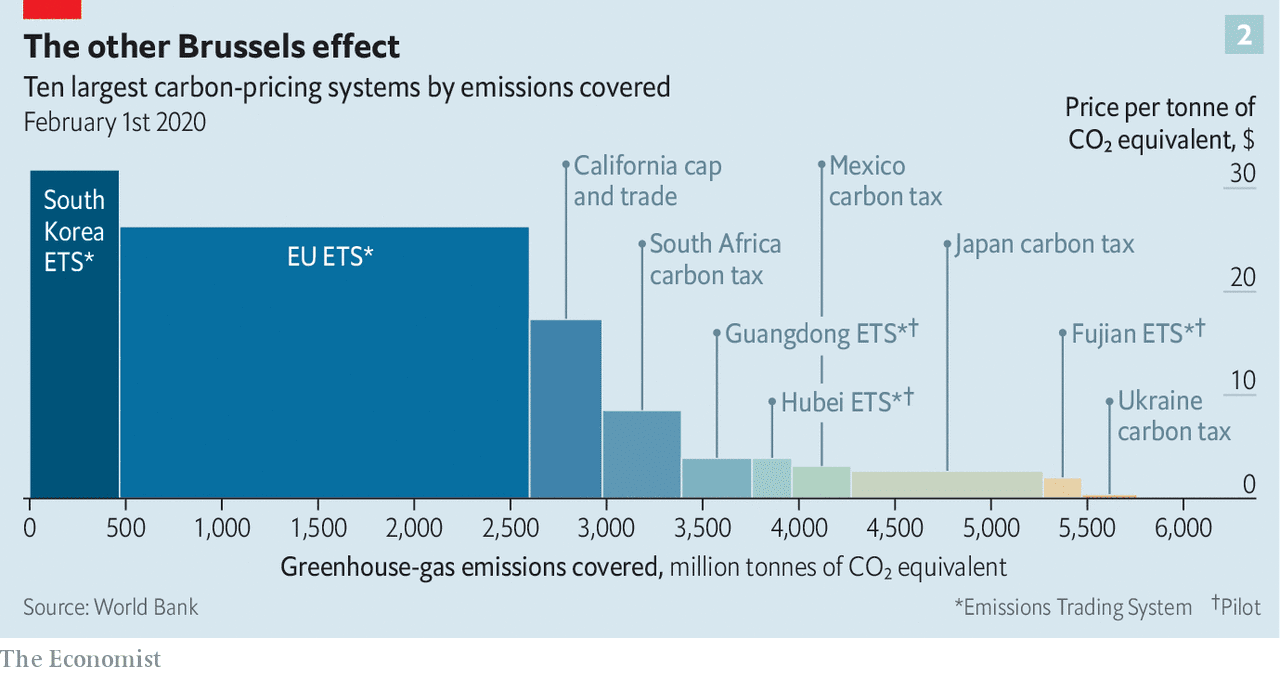
\includegraphics[scale=0.2]{photos/ets.png}
    \caption{Largest Emissions Trading Schemes}
    \label{fig:ets}
\end{figure}

Carbon prices are open to government manipulation from centralised
authorities and are often the subject of heated debates. An example
was the `axe the tax' campaign resulted in the abolishment of
the Australian ETS in 2014~\cite{EconE}. Moreoever, there is often
debate over where the money associated with carbon prices will go
- particularly in the case where an auction for carbon credits occurs.
If money raised from an ETS is used to lower taxes elsewhere then
opponents on the left of politics accuse the policy of not actively
fighting climate change. Generally, opponents on the right accuse carbon
prices of stifling economic growth - an example of an unecessary
government overreach.

The blockchain, which acts as an immutable ledger, has the potential to
deliver `trust' into the market for carbon. As opposed to being run
by a centralised authority like the government, it can instead be run
openly on the blockchain visible to all participants in the market for
carbon. Therefore, the openness of a blockchain ETS can be used to combat
its most fierce criticsm - which is its usage as a political tool.
A blockchain ETS can be designed so a `fee-and-dividend' is used, meaning
the distribution of payments can go straight back to the people thereby
incentivising long-term adoption~\cite{EconE}.

I will use the rapidly growing Hydrogen energy market - with its novel Hydrogen
certification process - to show how producers can pay for accrued
negative externalities. Hydrogen certificates can be automatically
submitted with a level of recorded emissions, whereby tokens are deducted
from a producer's carbon account upon submission. Smart contracts
(programs on the blockchain) will be used to represent the logic
of an ETS targetting hydrogen energy producers.

\section{Hydrogen Certificates}
The hydrogen market is a growing form of energy production created
from resources such as natural gas, coal, solar and wind. Hydrogen is
deemed a `clean fuel' because when it is consumed in a fuel cell
only water is produced. The hydrogen market is particularly important
for Australia since the industry is expected to create up to 7,600 jobs
and contribute \$11 billion a year to GDP~\cite{coag}. As part of an
effort to reduce cumbersome regulation associated with Hydrogen
markets internationl standards have been developed. Moreoever,
standards embedded into a \textit{hydrogen certificate} can
assist to manage the lifecycle of hydrodgen and ensure carbon
is not being emitted. As of 2020, there are eight international
hydrogen standards (see Table~\ref{tab:standards})
defining features such as safety and quality~\cite{stan}.

\begin{table}[H]
    \centering
    \begin{tabular}{|l|l|}
        \hline
        \multicolumn{1}{|c|}{\textbf{Standard}} & \multicolumn{1}{c|}{\textbf{Description}}            \\ \hline
        AS 16110.1:2020                         & Safety                                               \\ \hline
        AS ISO 16110.2:2020                     & Performance                                          \\ \hline
        AS ISO 14687:2020                       & Fuel Quality                                         \\ \hline
        AS 22734:2020                           & Industrial, commercial, and residential applications \\ \hline
        SA TS 19883:2020                        & Safety of pressure swing adsorption systems          \\ \hline
        AS ISO 16111:2020                       & Transportation                                       \\ \hline
        AS ISO 19881:2020                       & Gaseous hydrogen                                     \\ \hline
        AS 19880.3:2020                         & Gaseous hydrogen – Fuelling stations                 \\ \hline
    \end{tabular}
    \caption{International Hydrogen Standards}
    \label{tab:standards}
\end{table}
To help develop standards, centralised certification authorities
are being developed to act as certification schemes for hydrogen.
One of the most popular such schemes is CertifHy - a European
scheme for hydrogen certification~\cite{certifhy}. Centralised
certification schemes provide services such as the issuance of
hydrogen certificates along with the ability for users to create
an account to track the registry of owned certificates. Generally,
hydrogen certificates have the ability to detail technical information
along with crucial greenhouse gas information.

A key problem with the centralisation of certification authorities is the
lack of openness involved. Customers become reliant on a key provider to
conduct certification, fostering less `trust' in the market for hydrogen.
Due to a lack of trust, a blockchain-based approach to hydrogen
certification would allow for greater extensibility in the different
certificates available. Crucially, an ETS with on-chain energy
certification can enforce carbon prices in a market. For example,
if a hydrogen certificate has not paid for its carbon usage using
the on-chain ETS - then due to the immutability and openness of the
blockchain such a certificate could be marked as not valid for
trading inside a commodity-market. This thesis will make the
assumption that such a rigorous certification scheme exists, and will
outline how an ETS can be constructed to
make use of certificates created by producers thereby pricing carbon.

\section{Blockchain Emission Trading Schemes}
\subsection{Bitcoin-based ETS}
An early adoption of blockchain carbon pricing was the
creation of a bitcoin-based emissions trading infrastructure model
in 2015~\cite{vic15}. The model proposed a blockchain called
Decentralised Carbon Emissions Trading Infrastructure (D-CETI)
inheriting a significant amount of the innovations created with
Bitcoin by Satoshi Nakamoto in 2009. The authors proposed that
the significant barriers limiting the effectiveness of the
major ETS schemes (EU ETS) was the lack of security and privacy
participants face in cardbon trading~\cite{vic15}. As a solution,
Bitcoin's at the time novel approach to security using hashed
transactions and computationally difficult hash puzzles was deemed by the
authors as an appropriate solution to the shortcomings of
the large ETS schemes.


\begin{figure}[H]
    \centering
    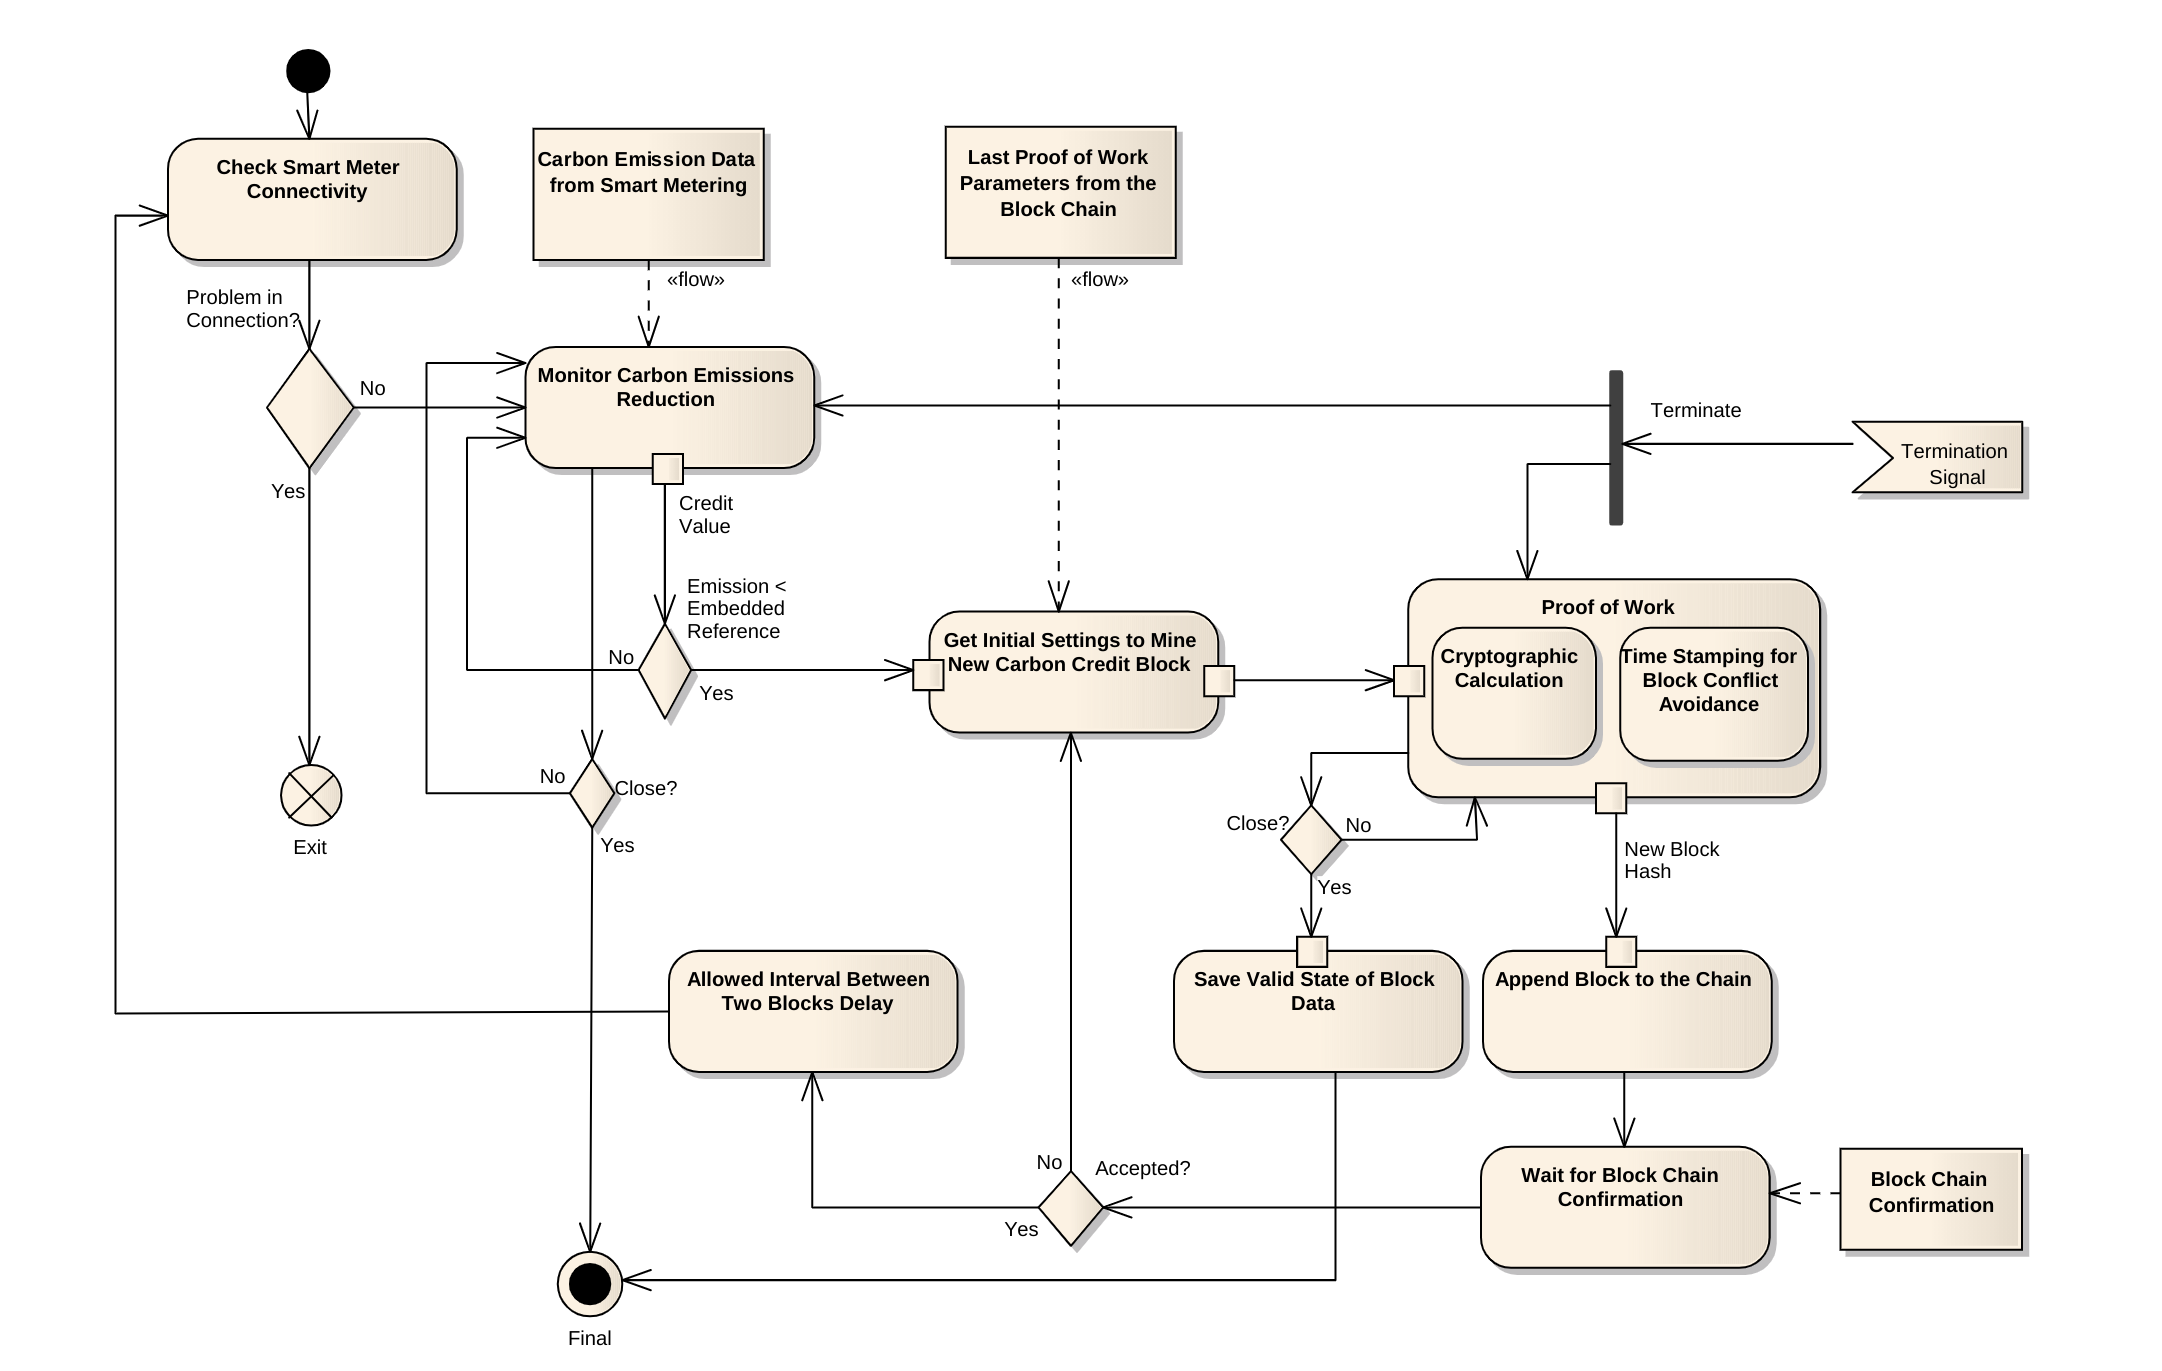
\includegraphics[scale=0.38]{photos/bitcoin.png}
    \caption{Bitcoin-based ETS}
    \label{fig:btc}
\end{figure}

In principal, the bitcoin-based ETS proposed functionality for
users to generate carbon tokens, register, sell,
and bid for credits. As a result, the system for a carbon market
was almost identical to the cryptocurrency Bitcoin with the
primary difference being the use of an ETS focused coin.
To deal with the throughput demands for an active ETS market,
the block generation rate on the chain became one block
every 150 seconds in contrast to Bitcoin's one block every
600 seconds~\cite{vic15}. Moreoever, participants in the bitcoin ETS market
would have to generate new blocks through miners solving cryptographic hash
puzzles (see Figure~\ref{fig:btc}).

The downsides to the bitcoin-based ETS are significant - the
throughput of the system is too low to ever be usable in an active
ETS market. Although increasing the throughput from 7 transactions
per second (TPS) for Bitcoin to roughly 28 TPS, such a solution
still relies on computationally expensive mining to achieve
system consensus~\cite{vic15}. Moreoever, Bitcoin's reliance on
hash puzzles requires the continuous consumption of carbon emitting
energy - potentially worsening the market failure which the ETS is aiming to
remedy.

The bictoin-based ETS relies on a primitive form of smart contracts
inherited from \textit{Bitcoin Script} - meaning the smart contracts
are not turing complete. Therefore, it would not be possible to
express detailed business logic such as the auctioning of tokens
or custom carbon prices into such an architecture. Simply stated -
a Bitcoin-based ETS is insufficient for a carbon market.